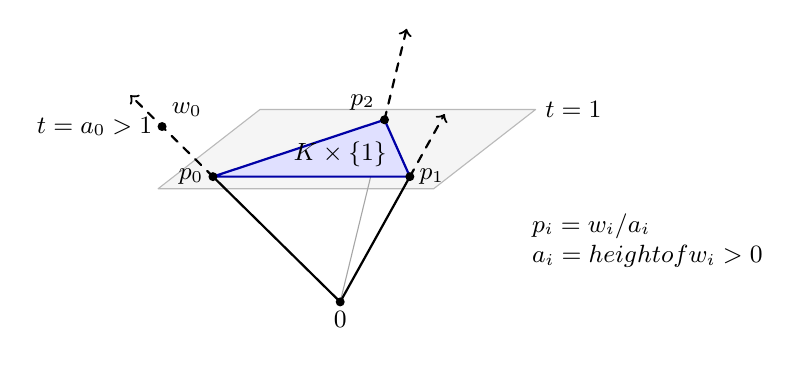
\begin{tikzpicture}[scale=1.25,
    x={(1cm,0cm)},y={(0.45cm,0.35cm)},z={(0cm,1.5cm)},
    line cap=round,line join=round,font=\small]
  \coordinate (O) at (0,0,0);
  \coordinate (P0) at (-1,-0.65,1);
  \coordinate (P1) at (1,-0.65,1);
  \coordinate (P2) at (0,1,1);
  \coordinate (W0) at (-1.4,-0.91,1.4);
  \fill[gray!8] (-1.4,-1,1)--(1.4,-1,1)--(1.4,1.3,1)
    --(-1.4,1.3,1)--cycle;
  \draw[gray!55] (-1.4,-1,1)--(1.4,-1,1)--(1.4,1.3,1)
    --(-1.4,1.3,1)--cycle;
  \node[anchor=west] at (1.4,1.3,1) {$t=1$};
  \draw[gray!70] (O)--(P2);
  \fill[blue!12] (P0)--(P1)--(P2)--cycle;
  \draw[blue!65!black,thick] (P0)--(P1)--(P2)--cycle;
  \draw[thick] (O)--(P0) (O)--(P1);
  \draw[thick,dashed,->] (P0)--(-1.65,-1.0725,1.65);
  \draw[thick,dashed,->] (P1)--(1.5,-0.975,1.5);
  \draw[thick,dashed,->] (P2)--(0,1.5,1.5);
  \fill (W0) circle[radius=1.3pt]
    node[above right] {$w_0$} node[left] {$t=a_0>1$};
  \fill (O) circle[radius=1.3pt] node[below] {$0$};
  \fill (P0) circle[radius=1.3pt] node[left] {$p_0$};
  \fill (P1) circle[radius=1.3pt] node[right] {$p_1$};
  \fill (P2) circle[radius=1.3pt] node[above left] {$p_2$};
  \node at (0,0,1) {$K\times\{1\}$};
  \node[align=left,anchor=west] at (2.3,-1,0.65)
    {$p_i=w_i/a_i$\\$a_i=\text{height of }w_i>0$};
\end{tikzpicture}